\documentclass{beamer}
\usetheme{Warsaw}

\newcommand{\<}{\langle}
\renewcommand{\>}{\rangle}

\title{Weighted Finite State Transducers}
\author{Ilya Edrenkin and Georgy Bronnikov}
\date{October 24, 2012}

\begin{document}

\maketitle

\section{Definitions and preliminaries: (10--15~min.)}

\begin{frame}
  \begin{itemize}
  \item Finite State Automaton (FSA)
    \begin{itemize}
    \item definition
    \item main applications
    \end{itemize}
  \item Weighted Finite State Automaton (WFSA)
    \begin{itemize}
    \item definition
    \end{itemize}
  \item Finite State Transduser (FST)
    \begin{itemize}
    \item definition
    \end{itemize}
  \item Weighted Finite State Transducer (WFST)
    \begin{itemize}
    \item definition
    \item advantages over WFSA
      \begin{itemize}
      \item composability
      \item invertibility
      \end{itemize}
    \item equivalence
    \end{itemize}
  \item Digression: Semirings
    \begin{itemize}
    \item definitions
    \item examples
    \end{itemize}
  \end{itemize}
\end{frame}

\subsection{Finite State Automata}
\begin{frame}
  \frametitle{Finite State Automata: Definition}

Finite-State Automaton (Machine) is an abstract model of computation. FSA is defined by the following elements:

      \begin{itemize}
      \item $\textit{Q}$ - finite set of states
      \item $\textit{I}\subseteq\textit{Q}$ - set of initial states
      \item $\textit{F}\subseteq\textit{Q}$ - set of final states
      \item $\textit{E}$ - finite set of pairwise oriented transitions between the states
      \item $\textit{A}$ - input alphabet
      \end{itemize}
\end{frame}
\begin{frame}
  \frametitle{Finite State Automata: State Diagram}

Hence, FSA can be naturally represented as an oriented graph. FSA is said to \textit{accept} an input string if the transitions corresponding to this string form the path from initial to final states.
\begin{center}
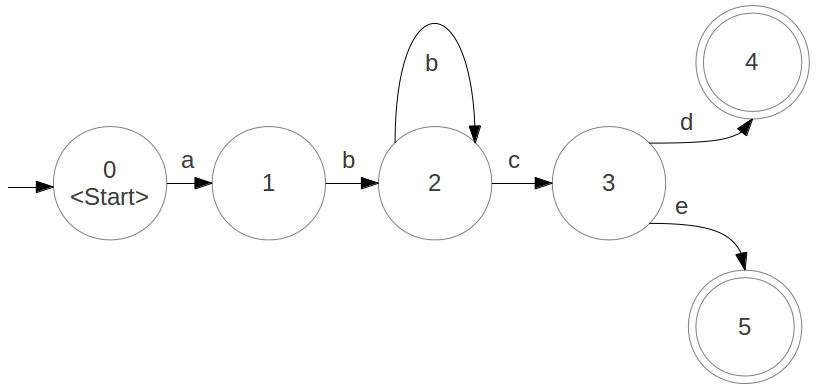
\includegraphics[width=6cm]{fsa-regexp-1.png}\\
\end{center}
This automaton accepts strings that match to the regular expression a(b*)c(d$\mid$e). The final states 4 and 5 are marked with a double circle.
\end{frame}
\begin{frame}
  \frametitle{Weighted Finite State Automata}

Let's assume that transitions might be different, say, more or less difficult to go through. This introduces the concept of weights.
\begin{center}
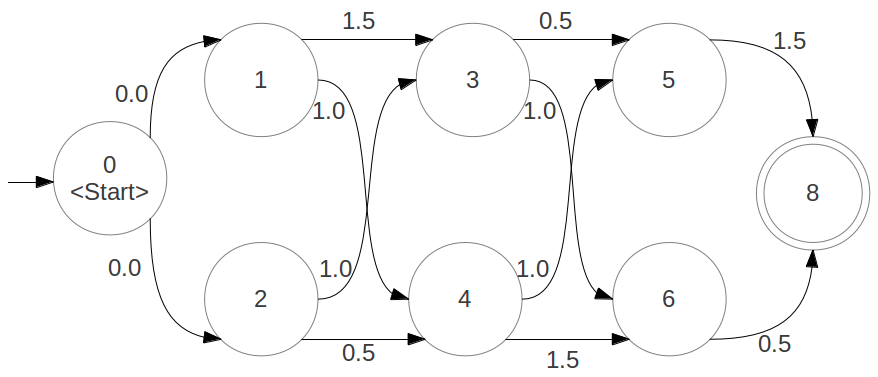
\includegraphics[width=6cm]{fsa-weights-2.png}\\
(input labels omitted)
\end{center}
This automaton is \textit{weighted}. Each transition is associated with a number, which can represent its probability, desirability, cost, etc.
\end{frame}
\begin{frame}
  \frametitle{Finite State Automata: Determinism}

FSA is said to be deterministic, if for each state there are no two output edges with the same label.
\begin{center}
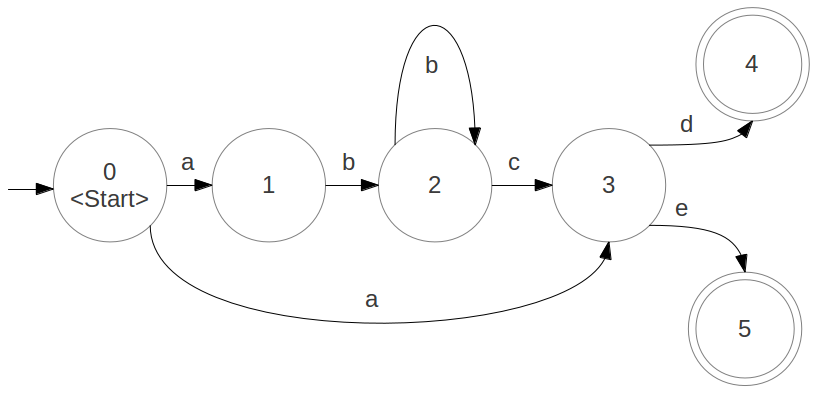
\includegraphics[width=6cm]{fsa-determination-3.png}\\
\end{center}
This automaton is \textit{non-deterministic}. State 0 has two output edges labeled with $a$.\\
\textbf{Claim}: each non-deterministic unweighted automaton can be efficiently determinized.
\end{frame}
\begin{frame}
  \frametitle{Finite State Transducers: Definition}

A \textit{Finite-State Transducer} (FST) is basically a FSA with an output string.
\begin{center}
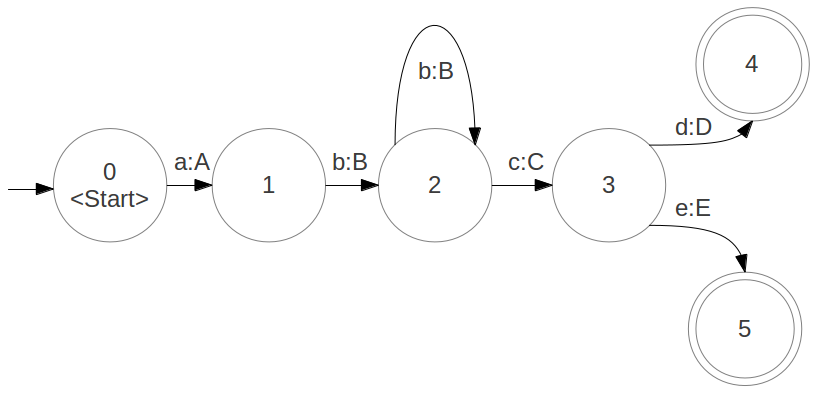
\includegraphics[width=6cm]{fst-example-4.png}\\
This FST simply outputs the uppercase version of the input string.
\end{center}
Output labels of FST are defined over the alphabet $B$.
\end{frame}
\begin{frame}
  \frametitle{Weighted Finite State Transducers}
\begin{itemize}
\item A Weighted Finite-State Transducer (WFST) is a FST with weighted edges.
\item It can be either deterministic or not.
\item Two WFSTs are said to be \textit{equivalent} if they associate the same output string and total weight to each input string.
\item WFST is said to be \textit{minimal} if there is no equivalent WFST with a smaller number of states.
\end{itemize}
\end{frame}
\begin{frame}
  \frametitle{Weighted Finite State Transducers}
\begin{itemize}
\item A Weighted Finite-State Transducer (WFST) is a FST with weighted edges.
\item It can be either deterministic or not.
\item Two WFSTs are said to be \textit{equivalent} if they associate the same output string and total weight to each input string.
\item WFST is said to be \textit{minimal} if there is no equivalent WFST with a smaller number of states.
\item WFSTs can be determinized, minimized, and composed with each other.
\end{itemize}
\end{frame}
\begin{frame}
\frametitle{Semirings}
The weights of WFST are determined over a \textit{semiring}.\\
A semiring is a set R equipped with two binary operations - summation $\oplus$ and multiplication $\otimes$, such that:
\begin{itemize}
\item Summation is commutative monoid and has identity 0;
\item Multiplication is monoid and has identity 1;
\item Multiplication distributes over summation: a$\otimes$(b $\oplus$ c) = (a$\otimes$b) $\oplus$ (a$\otimes$c)
\item Multiplication by 0 annihilates R: 0$\otimes$a = a$\otimes$0 = 0
\end{itemize}
\end{frame}
\begin{frame}
\frametitle{Semiring examples}
Given this definition, different semirings can be considered.
\begin{center}
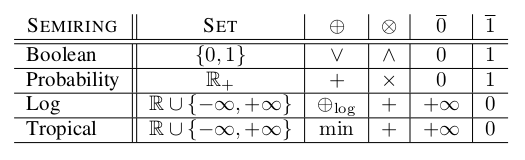
\includegraphics[width=6cm]{semiring-example-5.png}\\
\end{center}
Semirings are convenient for various dynamic programming approaches.
\end{frame}




\section{Basic component WFSTs used in speech recognition (7--10~min.)}
\begin{frame}
  \begin{itemize}
  \item Acoustic model
  \item Lexicon
  \item Grammar
  \end{itemize}
\end{frame}
\section{WFST production algorithms (20-25~min.)}

\subsection{Composition}

\begin{frame}
  \frametitle{Composition}

  Given a WFST $T_1$ from input alphabet $\mathcal{A}$ to output alphabet
  $\mathcal{B}$, and $T_2$ from $\mathcal{B}$ to $\mathcal{C}$, produce a WFST $T_1 \circ
  T_2$ from $\mathcal{A}$ to $\mathcal{C}$, such that the results of applying $T_1
  \circ T_2$ to a string $s \in \mathcal{A}^*$ is equivalent to the results of
  first applying $T_1$ to the same string, then running $T_2$ over the
  results (the same output strings receive the same weight).
\end{frame}

\begin{frame}
  \frametitle{The case without empty transitions}

  Basically, a cartesian product of the two transducers.

  Let 
$$
\begin{array}{ll}
T_1 = \<\mathcal{A}, \mathcal{B}, Q_1, I_1, F_1, E_1, \lambda_1, \rho_1\> &
  \mbox{and} \\
T_2 = \<\mathcal{A}, \mathcal{B}, Q_2, I_2, F_2, E_2, \lambda_2, \rho_2\> \\
\end{array}
$$
Then
$$
T_1 \circ T_2 = \<\mathcal{A}, \mathcal{C}, Q, I, F, E, \lambda, \rho\>
$$
where
$$
\begin{array}{rcll}
  Q & = & Q_1 \times Q_2 \\
  I & = & I_1 \times I_2 \\
  F & = & F_1 \times F_2 \\
  E & = & \{\<\<s_1,s_2\>, w_1 \otimes w_2, \<t_1, t_2\>\> \; | \; \<s_1,w_1,t_1\>
              \in E_1, \<s_2, w_2, t_2\> \in E_2\} \\
\end{array}
$$
$$
\begin{array}{rcll}
  \lambda[\<q_1,q_2\>] & = & \lambda_1[q_1]\otimes\lambda_2[q_2] & \mbox{for
    all $q_1 \in I_1$, $q_2 \in I_2$} \\
  \rho[\<q_1,q_2\>] & = & \rho_1[q_1]\otimes\rho_2[q_2] & \mbox{for
    all $q_1 \in F_1$, $q_2 \in F_2$} \\
\end{array}
$$
\end{frame}

\begin{frame}
  \frametitle{Empty transitions}

  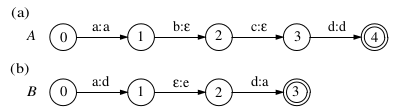
\includegraphics[width=4cm]{composition-example-1.png}\\
  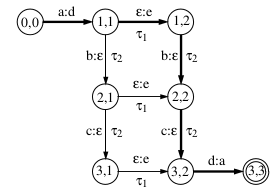
\includegraphics[width=4cm]{composition-example-2.png}

\end{frame}

\subsection{Determinization}
\begin{frame}
  \begin{itemize}
  \item Algorithm for an WFSA
  \item Applicability (what happens to a WFST?)
  \end{itemize}
\end{frame}

\subsection{Minimization}

\begin{frame}
  \begin{itemize}
  \item Weight pushing. Problems with computing potentials.
  \item Minimization itself
  \end{itemize}
\end{frame}






\section{WFST use algorithms (10-15~min.)}

\begin{frame}
  \frametitle{Dynamic programming}
  Conveyor problem: find the shortest way to finish an assembly, given two different assembly lines and transitions between them. 
  \begin{center}
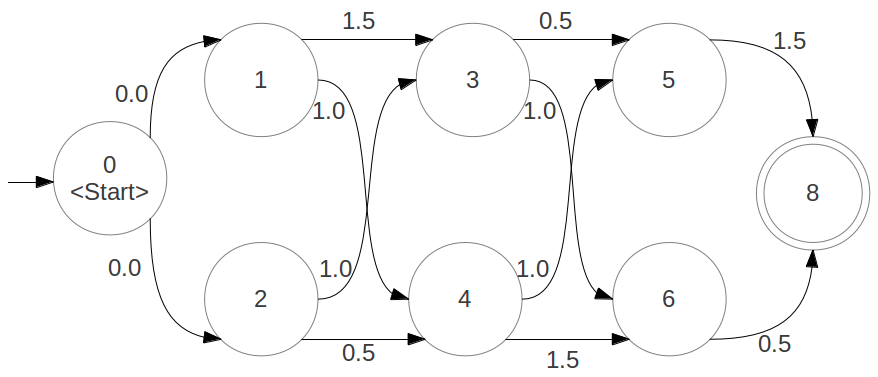
\includegraphics[width=6cm]{fsa-weights-2.png}\\
The weights represent assembly times.
\end{center}
This problem is easily solved with min-sum approach.
\end{frame}

\begin{frame}
  \frametitle{Viterbi}
  Suppose we have a fully specified HMM with known transition and emission probabilities. How do we recover the most probable sequence of hidden model states given the output?
    \begin{itemize}
  \item For each time frame we have the same N states.
  \item For each state we have constant emission probabilities for each symbol.
  \item We also have constant transition probabilities from state to state between the adjacent time frames.
  \end{itemize}
So we can build such a conveyor, where states are "assembly lines", transition probabilities are assigned to the edges, and emission probabilities are located in vertices.
\end{frame}

\begin{frame}
  \frametitle{Viterbi Max-Sum}
      \begin{itemize}
\item The probability of a particular path is simply a multiplication of the corresponding transition and emission probabilities through the automaton (or summation, if logprobs are used).
\item We simply use max-sum approach to determine the most probable sequence of model states that generated the observed output.
\item More accurate estimations of probabilities of each state at each time frame can be obtained by Forward-Backward (or Belief Propagation) algorithms, that are quite similar in the approach.
\item Viterbi beam search and other modifications are used to improve the efficiency of the algorithm, although this does not guarantee optimal decisions.
  \end{itemize}
\end{frame}

\end{document}